\section{Geometric interpretation}\label{sec:geometric-interpretation}
Here is a geometric interpretation of the Grover algorithm, following from the observation that the quantum state~\ref{eq:initial-state} stays in a two-dimensional subspace after each step of the algorithm. We will show that the Grover iteration can be regarded as a rotation in the two-dimensional subspace spanned by the starting vector $\ket{\psi}$ and the state $\ket{\beta}$ consisting of a uniform superposition of solutions to the search problem. 

We shall adopt the convection that $\sum_{x}^{''}$ indicates a sum over all $x$ which are solutions to the search problem, and $\sum_{x}^{'}$ indicates a sum over all $x$ which are not solutions to the search problem. Define normalized states.

\begin{equation*}
\begin{split}
 \ket{\alpha} &\equiv \frac{1}{\sqrt{N-M}} \sum_{x}{}^{''} \ket{x} \\
 \ket{\beta} &\equiv \frac{1}{\sqrt{M}} \sum_{x}{}^{'} \ket{x}.
\end{split}
\end{equation*}
The initial state $\ket{\psi}$ may be expressed as:
\begin{equation*}
    \ket{\psi} \equiv \sqrt{\frac{N-M}{N}} \ket{\alpha} + \sqrt{\frac{M}{N}} \ket{\beta}
\end{equation*}

Although we do not know the value of $\beta$ we do know that 
\begin{equation}
    \abs{\braket{\beta | \psi}} = \sqrt{\frac{M}{N}} \equiv \sin{\frac{\theta}{2}}
\end{equation}
irrespective of the value of $\beta$. Were we to measure the state $\ket{\beta}$ by projecting onto the computational basis the probability that we would find the marked state $\ket{\beta}$ is only $1/N$.  However we can repeatedly iterate a transformation that enhances the probability amplitude of the unknown state $\ket{\beta}$ that we are seeking, while suppressing the amplitude of all of the
undesirable states $\ket{x} \neq \ket{\beta}$. This is done by the iteration of~\ref{eq:grover-iteration} as we are going to see.

Consider the subspace spanned by $\ket{\psi}$ and $\ket{\beta}$ and equivalently the subspace spanned by $\ket{\beta}$ and the orthogonal state $\ket{\alpha}$.
The algorithm begins with the initial ket $\ket{\psi}$, which lies in the subspace. The operator $\hat{U}_\beta$ is a reflection at the hyperplane orthogonal to $\ket{\beta}$ for vectors in the subspace spanned by $\ket{\alpha}$ and $\ket{\beta}$. This can be seen by writing $\hat{U}_\beta$ in the form of a Householder reflection\footnote{A Householder reflection is a linear transformation that describes a reflection about a plane or hyperplane containing the origin.}:

\begin{equation}\label{eq:beta-projection}
    \hat{U}_\beta = \hat{I} - 2 \ket{\beta}\bra{\beta}.
\end{equation}
We can see that $\hat{U}_\beta$ flips the sign of the state $\ket{\beta}$ but acts trivially on any state orthogonal to $\ket{\beta}$. Acting on any vector in the $2^n$ dimensional Hilbert space $\hat{U}_\beta$  reflects the vector about the hyperplane orthogonal to $\ket{\beta}$ as it preserves the component in the hyperplane and flips the component along $\ket{\beta}$. Note that the subroutine performs this reflection for this particular computational basis state $\ket{\beta}$ but we know nothing about the value of $\beta$.

 The operator $\hat{U}_\psi = 2 \ket{\psi}\bra{\psi} - \hat{I}$ is a reflection through $\ket{\psi}$; acting on an arbitrary vector it preserves the component along $\ket{\psi}$ and flips the compment in the hyperplane orthogonal to $\ket{\psi}$. Both operators $\ket{U}_\psi$ and $\ket{U}_\beta$ take states in the subspace spanned by $\ket{\alpha}$ and $\ket{\beta}$ to states in the subspace. 
 
 Let $\cos\theta/2 = \sqrt{(N-M)/N}$ so that $\ket{\psi} = \cos\theta/2\ket{\alpha} + \sin\theta/2\ket{\beta}$.  The effect of the two reflections is
 
 \begin{equation*}
    \hat{G}\ket{\psi} = \cos\frac{3\theta}{2} \ket{\alpha} + \sin\frac{3\theta}{2} \ket{\beta}
\end{equation*}

so the rotation angle is in fact $\theta$. $\hat{U}_\beta$ reflects $\ket{\psi}$ in the plane about the axis $\ket{\alpha}$ and $\ket{U}_\psi$ reflects a vector about the axis $\ket{\psi}$. Together the two reflections rotate the vector by $\theta$. The Grover iteration, then, is nothing but a rotation by $\theta$ in the space determined by $\ket{\beta}$ and $\ket{\psi}$.

It follows that continued application of $G$ takes the state to:
\begin{equation*}
    \hat{G}^{k}\ket{\psi} = \cos\biggl(\frac{2k+1}{2}\theta\biggr) \ket{\alpha} + \sin\biggl(\frac{2k+1}{2}\theta\biggr) \ket{\beta}
\end{equation*}

The product of two reflections is a rotation. Therefore, the state space stays in this subspace for the entire algorithm (i.e. $G^k\ket{\psi}$ remains in the subspace spanned by $\ket{\alpha}$ and $\ket{\beta}$ for all $k$). 

\begin{figure}
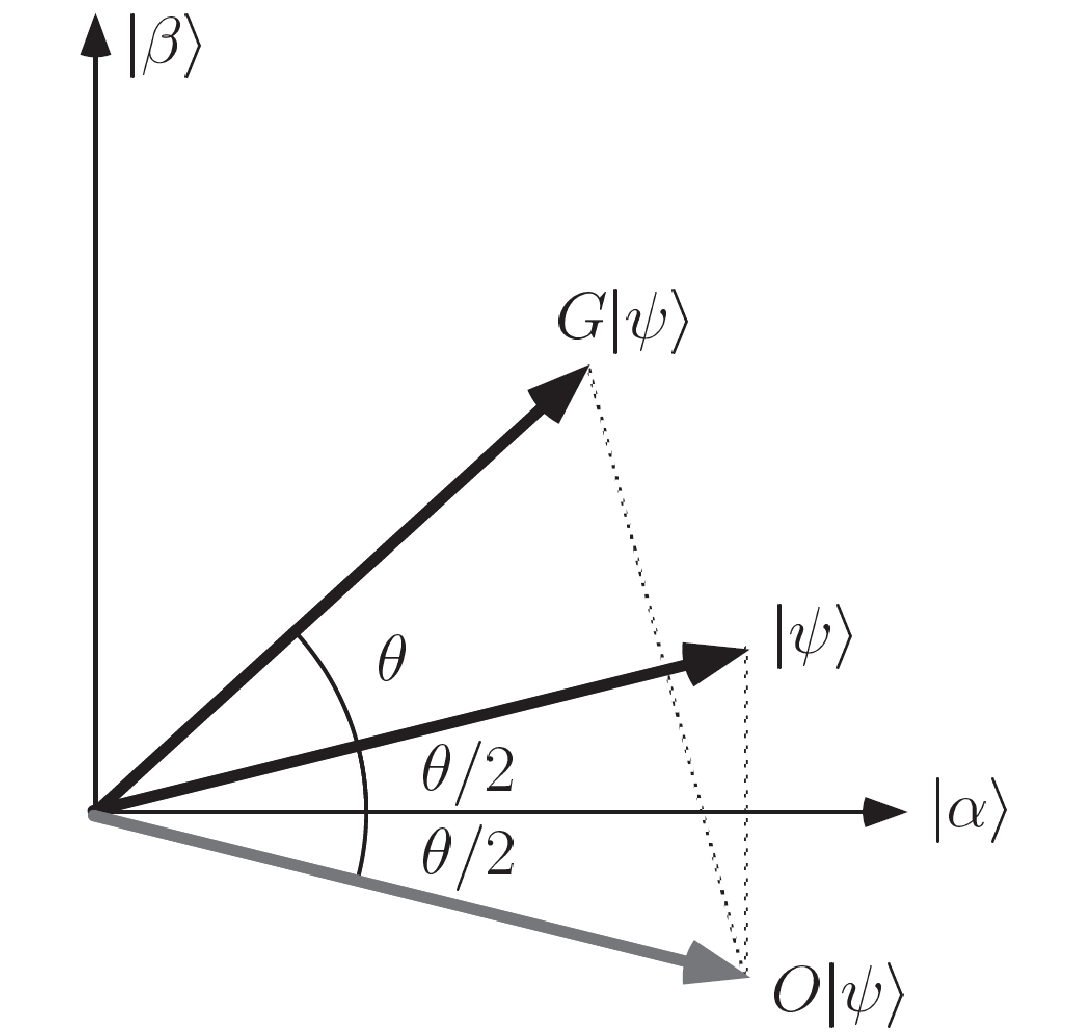
\includegraphics{geometric-interpretation.png}
\centering
\caption{The geometric interpretation of the first iteration of Grover's algorithm.}
\label{fig:geometric-interpretation}
\end{figure}

Repeated application of the Grover iteration rotates the state vector close to $\ket{\beta}$ as figure~\ref{fig:geometric-interpretation} shows. When this occurs, an observation in the computational basis produces with high probability one of the outcomes superposed in $\ket{\beta}$, which is the solution.

